% hello.tex - Our first LaTeX example!

\documentclass{article}

\usepackage{graphicx}
\usepackage[margin=1in]{geometry}
\usepackage{mathtools}
\usepackage{fancyvrb}
\DefineVerbatimEnvironment{code}{Verbatim}{fontsize=\small}
\DefineVerbatimEnvironment{example}{Verbatim}{fontsize=\small}

\begin{document}

\begin{titlepage}
\thispagestyle{empty}
\title{B1 Engineering Computation Project \\ Wireless Communication Channels: \\
Characterisation using orthogonal functions}
\author{James Routley \\
    Trinity College, Oxford \\
    6th January 2013 \\
    \texttt{james.routley@trinity.ox.ac.uk}}
\date{\today}
\maketitle    

\end{titlepage}





\section*{Introduction}


The aim of this project is to investigate the statistical properties of Wifi systems operating indoors. We shall do this by using a set of orthogonal basis functions called \emph{Laguerre functions} to construct a mathematical model of the probability density function describing the attenuation caused by the scattering process in the wireless communication medium. 

The project starts by showing how orthogonality is a useful property and that Laguerre functions are orthogonal before moving on to 

%{unfinished}

\section{Orthogonality}

We can use orthogonal basis functions to model our data. Orthogonal basis functions, such as:

$${f(0) = a_0 + a_1x + a_2x^2 + a_3x^3 }$$

\noindent are used because we can add more $x$ terms without having to recalculate our previous coefficients. 

\subsection{Fourier Series}

A common orthogonal basis set Fourier series, the functions $cos(n \omega x)$ and $sin(n \omega x)$, for  $n = 0, 1, ... $  formed an orthogonal set when the inner product is defined by the integral over a period ${T = \frac{2\pi}{\omega}}$, divided by the period.



\subsection{Using Matlab to compute Fourier series}

\subsubsection{Reminder about Matlab functions}

We are given a function fs\textunderscore orthog.m which integrates Fourier basis functions over a period. We are asked to write some code, fs\textunderscore orthogtest.m, which calls this function for $cos(m x) \times cos(n x)$ for ${m = 0 \to 6}$ and ${n = 0 \to 6}$ and stores the result in a 2D matrix:

\begin{code}
coscos = zeros(7); %set up a 7x7 matrix of zeroes to store the integral results

for m = 0 : 6
    for n = 0 : 6
        coscos(m+1, n+1) = fs_orthog(1, 1000, m, n, 'cc'); 
    end
end
\end{code}


\noindent We later repeat this code to include $sin(m x) \times sin(n x)$ and $cos(m x) \times sin(n x)$

%{What is the reason for this failure?}

\subsubsection{Code to compute Fourier series coefficients}

To compute the Fourier series coefficients, we are given two pieces of code, fs\textunderscore Acoeff.m and fs\textunderscore Bcoeff.m which calculate the $ A_m $ and $ B_m $ coefficients respectively. These functions are called from a top level script, fs\textunderscore triangle.m to plot a graph of the Fourier series approximation of a periodic function. The periodic function, a triangle wave:



%\begin{equation}
$$
	f(x)=\begin{cases}
	1+2x  &\text{ for } -\frac{1}{2}<  x< 0 \\ 
	1-2x  &\text{ for }  \:\:\:\:\:\:0<  x< \frac{1}{2}  
	\end{cases}
$$
%\end{equation}


\noindent is generated by fs\textunderscore periodictriangle.m.

If we run fs\textunderscore triangle.m with $ 4 \ n $ terms, we obtain the plot:
\begin{center}
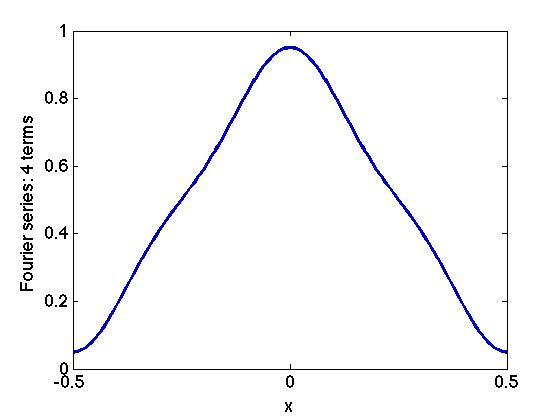
\includegraphics[scale=0.5]{fs_triangle4.jpg}
\end{center}


\begin{figure}[ht]
\centering
	\begin{minipage}[c][][b]{0.45\linewidth}
		\begin{center}
		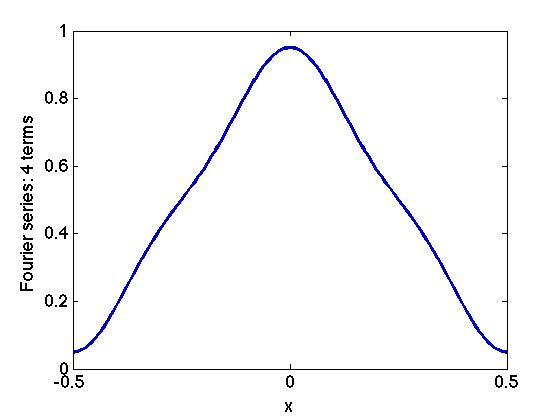
\includegraphics[scale=0.35]{fs_triangle4.jpg}  
		\end{center}
		\caption[b]{Normalised Gram Schmidt functions up to $n=5$.}
		\label{fig:minipage1}
	\end{minipage}
\quad\quad\quad\quad
	\begin{minipage}[c][][b]{0.45\linewidth}
		\begin{center}
		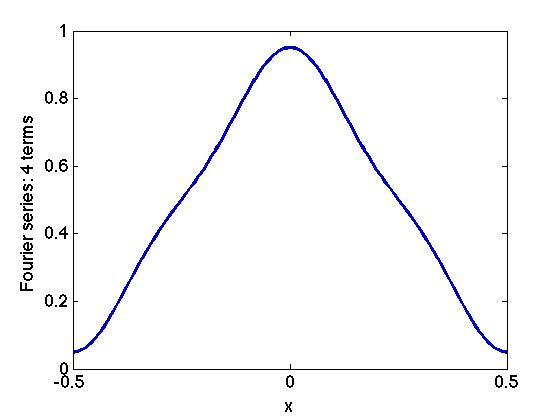
\includegraphics[scale=0.35]{fs_triangle4.jpg}
		\end{center}
		\caption[b]{$e$ coefficients up to $n=5$. HELKHWFLEHSOIDHFSOIDHFOSDIH}
		\label{fig:minipage2}
	\end{minipage}
\end{figure}


%{INSERT GRAPHS}

To judge the quality of the Fourier approximation as the number of $ n-terms $ changes, I wrote a function fs\textunderscore triangleerror.m which compares the least square error between the Fourier approximation and the actual triangle as the number of $ n-terms $ varies. 

I created a new function fs\textunderscore periodictrianglenew.m which generates the periodic function:

%{INSERT GRAPH}


%{- **Explore the number of terms required to provide a decent representation of the function as a gets smaller.** **How might you define decent** **What do you notice about the Bm coefficients**}

\section{Orthogonal Functions}
\subsection{The Gram-Schmidt Process}
1. explain the mathematics behind your method,
2. describe your implementation and supply the key parts of the code,
3. write clearly how to run your code,
4. describe the computational experiments you designed and performed to verify its performance,
5. give results, and importantly,
6. draw conclusions.


The Gram-Schmidt process is a method of orthogonalising a set of linearly independent functions. To do so, we take the 0th function and orthogonalise the rest of the functions in relation to it. We subtract a projection of the 0th function onto the 1st function from the 1st function. We repeat this with the 2nd function, subtracting projections of the 0th and the 1st functions from it, and so on. This can be represented mathematically:
$$
\begin{aligned}
g_0(x) &= v_0(x) \\
g_1(x) &= v_1(x) -e\_{10}g_0(x) \\
g_2(x) &= v_2(x) -e\_{20}g_0(x) -e_{21}g_1(x) \\
\end{aligned} \\
$$

This gives us an orthogonal basis set of functions $ g_0(x),\ g_1(x),\ g_2(x),\ ...$.

The $e$ values are the coefficients representing the projections of function onto each other. They can be calculated:

$$ e_{10} =  \frac{\langle v_1, g_0 \rangle}{\langle g_0, g_0 \rangle} $$

\subsection{An Important Example}

We are to perform Gram\textunderscore Schmitt orthogonalisation on the linearly independent set of monomials:

$$
\begin{aligned}
v_0(x) &= 1 \\
v_1(x) &= x \\
v_2(x) &= x^2 \\
\ldots
\end{aligned} \\
$$


with respect to the inner product:

$$ 
\langle g_n, g_m \rangle = \int_0^\infty \ g_n(x)g_m(x)e^{-x} \, \mathrm{d}x 
$$

My code is run by calling a top level script, gs\textunderscore script.m. The parameters of how many monomials to linearise and the range of x values to look at are defined within the script. The script calls on a series of functions to complete small tasks:

\begin{enumerate}
  \item Generate a matrix, $G$, of the monomials.
  \item Perform Gram-Schmitt orthogonalisation upon the matrix G to produce a matrix of orthogonal functions, $V$ and a matrix of coefficients, $E$.
  \item Normalise $V$ and verify orthonormality of $\tilde{V}$
  \item Plot the orthonormal functions $\tilde{v_0},\ \tilde{v_1},\ \tilde{v_2},\ ...   $
\end{enumerate}

The Gram-Schmitt orthogonalisation is performed by a function gs\textunderscore gramschmittorthogonalisation.m:


\begin{code}

function [E, G] = gs_gramschmittorthogonalisation(V, n, x)

    E = zeros(n, n-1);			%create empty matrices E and G
    G = zeros(n, length(x));
    G(1, :) = V(1, :);			%Set g0 = v0

    for k = 1 : n-1
        G(k+1, :) = V(k+1, :);	%set gk = vk
        for l = 1 : k
            %calculate e and store it in E
            E(k+1, l) = gs_innerproduct(x, V(k+1, :), G(l, :)) / gs_innerproduct(x, G(l, :), G(l, :));
            %subtract the projection of previous functions from the function in question 
            G(k+1, :) = G(k+1, :) -  E(k+1, l) .* G(l, :);
        end
    end
end


\end{code}

The nested for loops %**unfinished**


The inner product is calculated in gs\textunderscore innerproduct.m using Matlab's trapz function:

\begin{code}
function [result] = gs_innerproduct(x, y1, y2)
    result = trapz(x, y1.*y2.*exp(-x));
end
\end{code}

\section{Laguerre}
\subsection{Laguerre Polynomials}

Laguerre polynomials are a set of polynomials which are orthogonal with respect to the exponential weighting function. They can be generated using the \emph{Rodrigues formula}:

$$
L_n^{(\alpha)}(x) = \frac{1}{n!} x^{-\alpha} e^x \frac{d^n}{dx^n}(x^{n+\alpha} e^{-x}),  %n \in  \mathbb{N}, \alpha \in \mathbb{R} 
$$

We can see that to calculate the $n^{th}$ derivative, this simplifies to:

%insert simplified maths

\subsection{Calculating Coefficients of the $n^{th}$ Laguerre Polynomial}

This is implemented in Matlab in the function l\textunderscore laguerrecoefficients.m

\begin{code}
function c = l_laguerrecoefficients(n, a)
    
    c = 1/factorial(n) .* binomials(n) .* fcoeff(n, a) .* gcoeff(n);
    
end
\end{code}

Running the code for $ n = 5 $ and $ \alpha = 1 $ produces the results $-0.0083,\  0.2500,\  -2.5000\  10.0000\  -15.0000\  6.0000$ as expected. 

\subsection{Calculating Laguerre Polynomials Recursively}

We then write code which successively computes the Laguerre polynomials up to order $ n $.

Our top level script, l\textunderscore recurrsivelaguerre.m calls upon the function l\textunderscore recurrsivelaguerrecoefficients.m to generate a matrix of Laguerre coefficients.  

\begin{code}

function C = l_recurrsivelaguerrecoefficients(n, a)

%set up matrix C
    C = zeros(n);
    C(1, n) = 1;
    C(2, n-1 : n) = [-1, a + 1];

%cycle through rows and calculate and store coefficients
    for i = 3:n
        
%caclculate the values of the coefficients of the recurring section of
%equation
        reccoeff1 = [-1 , (2*(i-1) + a -1)];
        reccoeff2 = ((i-1) + a -1);
        
%multiply the polynomials together using conv
        x = conv(reccoeff1, C(i-1, :));
        x(1) = [];          %corrects for syntax error caused by using conv
        y = conv(reccoeff2, C(i-2, :));
        
%subtract one polynomial from the other and store in C
        C(i, :) = 1/(i-1)*(x - y);
    end
end
\end{code}

The code uses the MATLAB function %'conv' to do the necessary multiplication of two polynomials. 

The script then generates generates a matrix of values representing the equations:

$$
\begin{aligned}
y &= 1 \\
y &= x \\
y &= x^2 \\
&\vdots \\
y &= x^n
\end{aligned} \\
$$

and multiplies the relevant equations with the relevant coefficients to generate the Laguerre Polynomials or order up to $ n $.

For $ n = 6 $ and $ \alpha = 0 $ we get:

%insert graph

\subsection{Comparison to your Polynomials}








\end{document}

